\chapter{Literature Review}\label{ch:literature}
\acresetall

\section{Stereo Sensing} \label{ch:literature:obstacle_avoidance:sensing:stereo_vision}

As mentioned in Chapter \ref{ch:intro}, a \ac{CAS} needs to accurately sense the surroundings in order to safely avoid the potential threats. Stereo vision uses a pair of synchronized cameras in order to capture a scene. The general idea is to infer distance to scene points by measuring parallax which is the object's position displacement when seen by two different angle of views \cite{cse_lecture}. That is, the difference in the captured pair of images can lead to an estimation of the object's distance. This difference in the position of two pixels which represent the same scene point is called \textit{disparity}.

In Figure \ref{stereo_setup} it is depicted the concept behind stereo vision \cite{Dijk}. The baseline between the two cameras is equal to B, the focal length of the cameras is equal to f and z is the distance of the obstacle. Here an assumption is made that they are perfect, linear, pinhole cameras. That means that distortion of the image has been removed, and projection of real-world points are linear. We can derive the equation that relates disparity with depth by using equal triangles \cite{Dijk}:

\begin{equation} \label{eq:disparity_depth}
d = B * f * z^{-1}
\end{equation}

\begin{figure}[]
  \makebox[\textwidth][c]{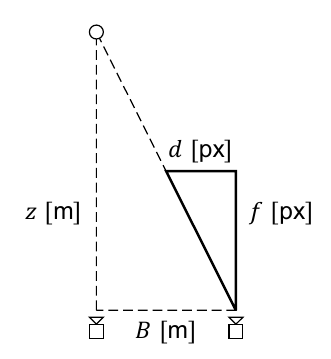
\includegraphics[width=0.4\textwidth]{2_background/images/stereo_setup.png}}
  \caption{Basic concept behind stereo vision, figure taken from \cite{Dijk}}
  \label{stereo_setup}
\end{figure}

If disparity is estimated correctly, then the depth image can be derived which relates every pixel in the captured frame with an estimated distance. That is, the accuracy of the stereo algorithm depends on the correct generation of a disparity map, which is its capacity to correctly match pixels between left and right image. This is rather a difficult process and many approaches have been developed over the years. 

Stereo vision disparity map algorithms can be classified into \textit{sparse }or \textit{dense }approaches.

\begin{description}
	\item[Sparse: ] \textit{Sparse }algorithms extract a number of keypoints and they try to match only this small number of points. Their accuracy depends on their ability to perform a good match between these points. Since a matching between all points is not performed the resulting depth map will contain large holes \cite{Dijk}.
	\item[Dense: ] \textit{dense }approaches try to match all the pixels and they compute the disparity image by finding the best disparity for every pixel. Consequently, all the points of the obstacles in the \ac{FoV} of the camera reprojected in the image space are assigned a disparity value. 
\end{description}

Stereo vision algorithms can be further classified into \textit{local }or \textit{global }approaches. 

\begin{description}
	\item[Local: ] A \textit{local }approach (also known are area based or window approach) computes the disparity of a given pixel by taking into account only the intensity values within a predefined support window \cite{Hamzah2016a}. Therefore, algorithms belonging in this category show low computational requirements and short run time.
	\item[Global: ] On the opposite to local approaches, \textit{global} methods try to minimize a global energy function in order to calculate disparity. This energy functions consists of a data term (takes into account the intensity of every pixel and its corresponding match) and a smoothness term (assumes that pixel of the same area should have similar disparity values) \cite{Hamzah2016a}. The main distinction between global approaches is the optimization procedure used. The main disadvantage of global approaches is that they are computationally expensive but can produce better results in texture-less environments.
\end{description}

  The analysis of the different categories makes clear that \textit{local} \textit{dense }approaches are the most suitable for drone sensing considering the needs for safety and low computational resources \cite{Dijk}. Here it should be mentioned that there are some algorithms which do not belong exactly to either category. The limitations of stereo vision is that it requires two cameras which results in a heavier set up and its limited range \cite{Pinggera2014} \cite{Dijk}. The accuracy of stereo algorithm depends mainly on its pixel matching method efficiency. 

%“textureless surfaces, finely or repetitively, textured surfaces, textures oriented parallel to the baseline, reflections and transparency, slanted surfaces and occlusions”\cite{Dijk}

\section{Collision Avoidance}\label{ch:literature:obstacle_avoidance:navigation}

In the previous section we described how the obstacles in the vicinity of the \ac{UAV} are detected. Since this work focuses on static environments the decision about whether a conflict is imminent or not is equivalent to the following question: ``Does the current trajectory pass through the detected obstacle?". Therefore, the collision detection process is simplified in this case. 

\textbf{\ac{UAV} collision avoidance} should successfully move the \ac{UAV} from an initial colliding state to a safe state. The path from the initial state to the safe state is calculated by a motion planning algorithm. In order to achieve this, knowledge of the surrounding environment is necessary. When collision avoidance is performed in unstructured environments, a map should be used in order to encode the world representation. These two components, the \textbf{motion planning} method and the \textbf{mapping} technique are the most essential parts in collision avoidance and determine the trajectory the UAV will follow to reach its goal state. An additional optional component is the usage of \textbf{dynamics }which permits high-speed flights. Similarly to stereo solutions, there is a plethora of approaches developed for collision avoidance.

\subsection{Path Planning}

In order to plan its avoidance maneuver, the \ac{UAV} needs to employ a motion planning algorithm and to have knowledge of the surrounding environment. Unfortunately, the term path planning in obstacle avoidance is often misused by implicitly assuming that it has to generate a trajectory towards a goal location. However, the real purpose of path planning in obstacle avoidance is to generate a maneuver or path that will prevent the \ac{UAV} from the upcoming collision. Reaching a goal state is a related but different matter that falls upon \ac{UAV} autonomous navigation and localization. In other words, there is a confusion between path planning for obstacle avoidance and path planning for autonomous navigation. 

An important criterion upon the decision of the path planning strategy is whether there is or not knowledge about the environment to which the flight will take place. 

\begin{description}
	\item[Global knowledge: ] Global knowledge assumes that the location of all obstacles is known.
	\item[Local knowledge:] Local knowledge of the environment assumes that the only information available is what the UAV captures through its sensing functionality, so the amount of information differs among different designs. 
\end{description}

The motion planning algorithms take into account the information encoded in a map and the complete or not knowledge of the environment to plan a trajectory or maneuver for the \ac{UAV} to execute when a collision is detected. They can be divided into two classes: \textit{reactive} and \textit{deliberative}. 

\begin{description}
	\item[Reactive: ]\textit{Reactive }planning executes a maneuver according to the presence of obstacles without having any other criterion except avoiding the imminent collision.
	\item[Deliberative: ] In \textit{Deliberative} planning a cost function is usually used to evaluate the different potential trajectories and find the optimized trajectory.
\end{description}

Usually, when \textit{global} knowledge is assumed, \textit{deliberative} planning is preferred since the environment is a-priori known and the application's main goal is to minimize the trajectory from the initial state to a goal state. In this case, localization is necessary as the problem of obstacle avoidance is simplified in the capacity of the drone to accurately localize itself. On the other hand, \textit{local }planning algorithms vary from \textit{reactive} to \textit{deliberative }ones. No matter the method used, the goal of the motion planning algorithm is always the same: generate a collision-free trajectory. In case the environment is unknown, there is no need for a complex path-planning technique.

\subsection{Mapping}\label{ch:literature:obstacle_avoidance:navigation:mapping}


The navigation of an \ac{UAV} takes place in the \textit{world space}, that is the ``physical space in which a \ac{UAV} exists" \cite{Goerzen2010a}. Everything \ac{UAV} acknowledges about its \textit{world space }should be encoded in this map. Every motion planning approach uses the information embedded in the map representation to generate a short or long term trajectory for the \ac{UAV} to follow. 

According to this study \cite{Dijk}, any kind of map should belong to one of the following categories: 

\begin{description}
	\item[Image-space: ]\textit{Image/Sensor space} maps is the simplest type of map. It is essentially the same as a depth map, that is the image captured by the camera has a depth value assigned to every pixel.
	\item[Discretized-space: ]\textit{Discretized }maps decompose the world space into smaller rectanguloid regions, i.e., a grid consisted of discrete cells that can be free or occupied. This mapping technique is not very efficient because the grid becomes very large when several dimensions are used . Moreover, it is not exact because there are cells that are half-free and half-occupied.
	\item[Continuous-space: ]Continuous-space maps estimate and store the exact position of the surrounding obstacles.
\end{description}

  
The choice of mapping puts some limits on drone navigation capabilities. \textit{Discretized-space} methods are very handful for application which require memory of previously examined areas such as exploration \cite{Brockers2016b}. This is impossible with \textit{image-space} methods, since they provide information usually restricted by the \ac{FoV} of the camera. Consequently, the \ac{UAV} may not be able to find its escape route through certain environments (e.g. labyrinth) \cite{Dijk}. However, \textit{discretized} maps have high memory and computational requirements, and are hence undesirable for low-cost platforms. Most obstacle avoidance solutions use 2-D or 3-D Cartesian probabilistic grid maps and every time an obstacle is detected it has to be projected from the image space to the Cartesian map \cite{Brockers2016b}. Consequently, the motion planning is performed directly on the built Cartesian map. Nevertheless, flights in maze-like environments are excluded, a less expensive solution would be an \textit{image-space} map. Finally, continuous-space maps are used for preventing collisions among \acp{UAV} \cite{Dijk}, therefore it is outside of the scope of this research.

Finally, two important decisions should also be taken after choosing a map category. The first one is the level of detail encoded in the map and the second one is is whether the map should combine multiple measurements in order to encode more information about its surroundings \cite{Dijk}. Even maps which belong to the same category may differ in a sense of their level of detail. For example, in \cite{Barry2018} they make use of an occupancy grid which encoded more details about the world space and is more computationally expensive than the octree-based search lattice used in \cite{Xu2015} while both approaches belong to the \textit{discretized space} category. Regarding the combination of multiple measurements, this feature would be very efficient for maze-like environments where there is a chance for the drone to get trapped. However, data fusion is a rather computationally expensive technique.

\subsection{Dynamics}

Any motion planning algorithm can potentially take into account dynamics by using a dynamic model of the \ac{UAV}. However, the first step of any obstacle avoidance implementation should be to first validate the efficiency of the approach in low-constant speed and subsequently make it more complex by adding kinematics and dynamics equations. By including dynamics in the navigation, it is ensured that the \ac{UAV} can indeed execute the generated maneuver to avoid the obstacle.

Dynamics may be taken into account explicitly or implicitly. For example, an approach that suggests the drone should move in a speed less than a predefined value takes implicitly dynamics into account. On the other hand, an approach that calculates the trajectory based on drone dynamics takes explicitly dynamics into account. The latter ones are more computationally expensive although not as computationally expensive as originally thought (e.g., \cite{Fragoso2017}). Even image-space approaches need the use of dynamics for high-speed flights. Dynamics of \ac{UAV} is a very particular topic on its own and outside of the scope of this research.

\section{State-of-the-Art Dense Stereo Algorithms and UAVs Stereo Studies}
\label{ch:literature:obstacle_avoidance:state_of_the_art_stereo}

In the following sections the state-of-the-art dense stereo algorithms will be presented. Moreover, low-cost stereo algorithms designed especially for obstacle avoidance will be briefly discussed.

\subsection{Dense Computer Vision Stereo Algorithms}

According to the taxonomy proposed in \cite{Scharstein2002} most stereo algorithms perform (subset of) the following steps:

\begin{enumerate}
	\item matching cost computation;
	\item cost (support) aggregation;
	\item disparity computation / optimization; and
	\item disparity refinement.
\end{enumerate}


In this section, a few important state-of-the-art computer vision algorithms are described, without presenting the employed disparity refinement (also known as post-processing) methods, since they are common in every stereo implementation. Instead, we focus on the way they generate the disparity values (steps 1-3).

\subsubsection{Block Matching}

Block Matching belongs to local-based methods and is probably the most intuitive and simplistic approach of stereo correspondence. It estimates disparity at a point by comparing a small region around that point with a similar-sized region extracted from the other image. For this comparison, many different classes of metrics can be used:

\begin{itemize}
	\item Correlation (\acs{NCC})
	\item Intensity difference (\acs{SAD}, \acs{SSD})
	\item Rank (\acs{RT}, \acs{CT})
\end{itemize}

\begin{figure}[H]
  \makebox[\textwidth][c]{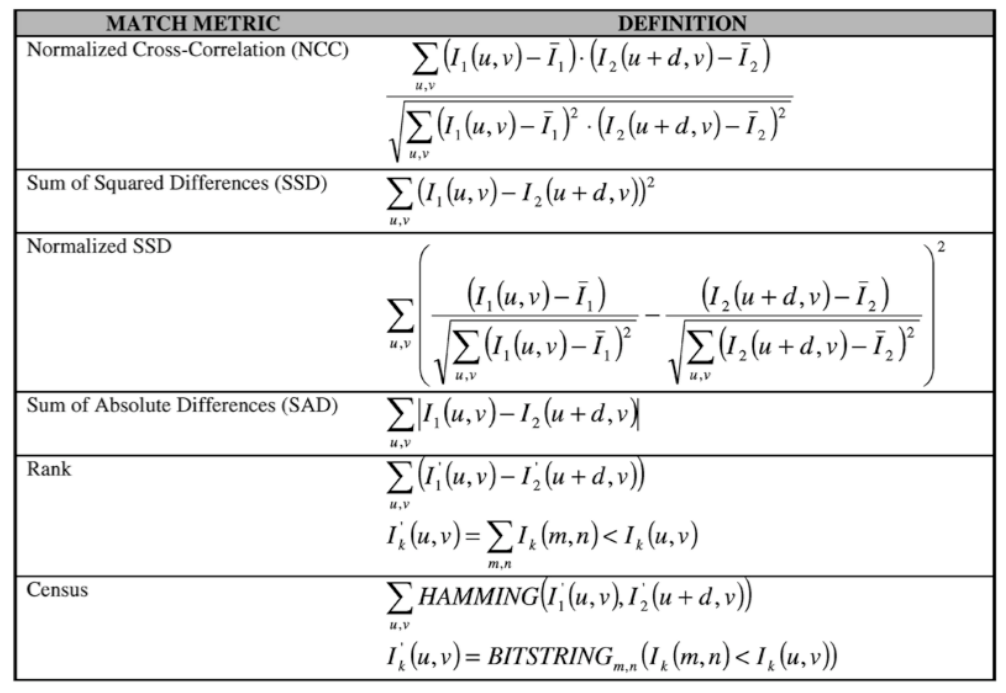
\includegraphics[width=0.7\textwidth]{2_background/images/block_matching_costs.png}}
  \caption{Basic block-matching costs - found in [lecture by Andrea Fusiello]\url{http://profs.sci.univr.it/~fusiello
}}
  \label{block_matching_costs}
\end{figure}


An extensive review and comparison of the metrics and aggregation methods that can be used for \acs{BM} can be found in \cite{Tombari2008a} \cite{Patil2013a}.

After assigning a cost to every disparity value, it decides upon the disparity of the pixel by performing a \acs{WTA} optimization. It simply selects the disparity value with the lowest cost. Finally, the disparity refinement vary according to the implementation. An example of a fast and effective implementation has been developed by Konolige \cite{Konolige1998}.

\subsubsection{Semi-Global Matching}

\ac{SGM} \cite{Hirschmuller2007} is a semi-global stereo algorithm and is known for being one of the most effective and accurate algorithms for disparity computation. It is essentially a combination of local and global approaches.

For pixelwise cost calculation, it uses either the \acs{BT} metric or \ac{MI} which shows tolerance in illumination change differences, though it is also more computationally expensive. As disparity computation based only on pixelwise costs is equivocal, it makes use of a cost aggregation method. That said, it aggregates matching costs in 1D from all directions equally. In order to calculate the total cost $S(\textbf{p},\textit{d})$ for a pixel \textbf{p} with disparity \textit{d}, it sums up the costs of all 1D paths. Finally, in order to select the disparity for the pixel of interest, it also follows the \acs{WTA} policy, i.e., it simply selects the disparity that corresponds to the lowest cost. A thorough analysis of this method, together with the recommended comparison metrics and disparity refinement methods are extensively described by Hirschmüller in \cite{Hirschmuller2007}. Note that there is a variant of this method called \ac{SGBM}, the only difference is that it uses also an extra window aggregation method like \ac{BM}.

\subsubsection{ELAS}

\ac{ELAS} \cite{Geiger2011} is a a Bayesian approach to stereo matching and achieves a good trade-off between accuracy and runtime. 

First of all, this algorithms computes the disparity values of only a set of strong support points. Since usually there are not many strong points in an image, the corners are also assumed to have a disparity equal to the disparity of their closest strong point. Subsequently, Delaunay triangulation, a prior and a maximum a-posteriori (MAP) estimation are used to calculate the disparities of the rest pixels.

\subsubsection{SPS-St}

\ac{SPS-St} \cite{Yamaguchi2014} is a two-stage approach that uses a classic stereo algorithm approach and a segmentation step subsequently. 

Initially, this approach uses a \ac{SGM} to construct a semi-dense depth map on the reference image. However, in comparison with the ``classic" \ac{SGM} algorithm, they use Cencus as a matching cost. The \ac{SGM} depth map is then ``used as input to the slanted plane method for inferring the segmentation, planes and boundary labels".



\subsection{Stereo In Obstacle Avoidance}
\label{ch:literature:state_of_the_art_stereo}

%(Note about this section: Should I keep these studies as an example of what exists out there? Or should I keep only the studies presenting novel stereo obstacle avoidance algorithms?)

As already mentioned in Chapter \ref{ch:intro}, stereo systems popularity surpasses single and multi camera approaches. Over the years, a great number of on-board stereo-based UAV studies has been developed. Some of them introduce a novel stereo algorithm especially designed for obstacle avoidance while others just use one of the classic computer vision stereo algorithms. The purpose of this section is to present the studies which introduce a novel stereo sensing approach specifically designed for low-cost, low-computational demanding obstacle avoidance and report the most popular stereo algorithms used in stereo-based obstacle avoidance studies. 

From the vast amount of stereo-based UAV studies only a few present a novel solution in a sense of designing a new stereo sensing approach targeting obstacle. In \cite{Byrne2006} they make use of the classic stereo algorithm \ac{BM} and extend it with a global segmentation step in order to increase robustness. This approach is similar to \ac{SPS-St} (the stereo corresponce is followed by a segmentation step) but with a lower computational intensive stereo correspondence (make use of \ac{BM} instead of \ac{SGBM}). For a 640 x 480 image they achieve a frame rate of 5-10 Hz while the stereo correspondence step runs at 23 Hz. However, they make use of a dedicated vision processor in order to achieve that performance. Their approach shows no false alarms and they do not present any avoidance strategy. Another study also uses \acs{BM} as the main component of their sensing block\cite{Barry2018}. Block Matching is used in order to estimate the distance of the obstacles in front but limit their search through distance to a single value. That said, they detect only obstacles that are placed in a certain-fixed distance away from the UAV (around 5 meters). The novelty in this approach is the integration of odometry information and previous single-disparity (in other words single-distance) results to recover missing depth information. While this approach significantly reduces computation load, there is a high risk of collision if the aircraft changes direction (e.g., turn left). If an obstacle exists in the new direction in a distance less than the chosen fixed detection distance, the obstacle will not be detected and a collision may occur. Finally, the most light-weight stereo approach performs stereo sensing on a 20-gram flapping wing \cite{DeWagter2014}. A line-based stereo algorithm is presented which significantly reduces computational requirements. It is the most computationally efficient stereo algorithm for dense-map generation as it was designed to run in a low-end STM32F405 (168 MHz) processor and still achieve a frame rate of 11 Hz on a full image of 128x96 pixels. The efficiency of this method has been tested only on sparse indoor obstacle environments.

Besides the few novel stereo sensing studies, there is a huge amount of stereo-based studies which present a complete obstacle avoidance solution (sensing and avoidance strategy) and make use of a classic computer vision stereo algorithm for sensing. The most popular algorithms used are \ac{BM} (e.g., \cite{Heng2011}, \cite{Meier2012}) and \ac{SGM} (e.g., \cite{Barrientos2011a}, \cite{Oleynikova2015a}, \cite{Ruf2018a}). 


%Through the study on the field, it should be noted that there is not yet defined an optimal stereo sensing solution for obstacle avoidance. High-speed implementations either require the usage of a hardware accelerator or make use of a simpler method thus paying a cost in their sensing accuracy. Moreover, a review of classic computer stereo vision approaches regarding their usage in \acp{UAV} misses from the existing literature. The most used algorithms so far are \ac{BM} and {SGM} and the latter one usually runs on a hardware accelerator (FPGA is the most popular one).

\section{State-of-the-Art Collision Avoidance Strategies}

In this section, first an attempt of classifying the different collision avoidance strategies is made and subsequently the state-of-the-art image-based techniques are presented.

\subsection{Classification of Collision Avoidance Approaches}
\label{ch:literature:obstacle_avoidance:navigation:classification}

The field of \ac{UAV} Collision Avoidance is relatively new and the last years has shown a rapid development. Because of that, there does not exist a clear-cut categorization of methods and many terms are misused. After examining the state-of-the-art literature on collision avoidance, we believe the following categories should be used: The navigation approaches can be divided in several categories based on the mapping technique (Image/Sensor space, Discretized space, Continuous space) \cite{Dijk}, knowledge of world space (local or global) and motion planning (reactive, deliberative). Consequently, when someone chooses a collision avoidance method, apparently a decision among all the different categories should be taken. Table \ref{table:navigation:classification} sum ups the advantages and disadvantages of each category. Several combinations among the categories can be made, while some combinations are de facto prohibited or preferably avoided (e.g., Image space mapping with Global environment knowledge).

% Please add the following required packages to your document preamble:
% \usepackage{multirow}
\begin{table}[]
\hskip-2.0cm\begin{tabular}{|c|c|l|c|l|}
\hline
\multirow{2}{*}{\textbf{Mapping}}                                                             & \textbf{\begin{tabular}[c]{@{}c@{}}Image/Sensor \\ space\end{tabular}}                                      & \multicolumn{1}{c|}{\textbf{Discretized space}}                                      & \multicolumn{2}{c|}{\textbf{Continuous space}}                                                                                                               \\ \cline{2-5} 
                                                                                            & \multicolumn{1}{l|}{\begin{tabular}[c]{@{}l@{}}- Low memory \\ - Low computational \\ complexity \end{tabular}}                                                                           & \multicolumn{1}{l|}{\begin{tabular}[c]{@{}l@{}}- Medium/High memory \\ - Medium/High computational \\ complexity \end{tabular}}                                                                                                                                            & \multicolumn{2}{l|}{\begin{tabular}[c]{@{}l@{}}- Low memory for\\  obstacle positions\\ - High memory for\\  cloud points\end{tabular}}                      \\ \hline

\rowcolor[HTML]{680100} 
\multicolumn{1}{l}{\cellcolor[HTML]{680100}{\color[HTML]{333333} }} & \multicolumn{1}{l}{\cellcolor[HTML]{680100}{\color[HTML]{333333} }} & \multicolumn{1}{l}{\cellcolor[HTML]{680100}{\color[HTML]{333333} }} & \multicolumn{1}{l}{\cellcolor[HTML]{680100}{\color[HTML]{333333} }} & \multicolumn{1}{l}{\cellcolor[HTML]{680100}{\color[HTML]{333333} }} \\ \hline                                                                                             
                                                                                                                                                                                         
                                                                                            
\multirow{2}{*}{\textbf{\begin{tabular}[c]{@{}c@{}}Knowledge of \\ Environment\end{tabular}}} & \multicolumn{2}{c|}{\textbf{Local}}                                                                                                                                                                & \multicolumn{2}{c|}{\textbf{Global}}                                                                                                                         \\ \cline{2-5} 
                                                                                              & \multicolumn{2}{l|}{\begin{tabular}[c]{@{}l@{}}- Low memory if previous sensing \\ measurements are discarded\\ - Medium/High memory if information \\is stored over time \\ - Trap situation may occur\\ - Possible local trajectory optimisation\end{tabular}} & \multicolumn{2}{l|}{\begin{tabular}[c]{@{}l@{}}- High memory\\ - High computational\\ complexity\\ - Possible global\\ trajectory optimisation\end{tabular}} \\ \hline

\rowcolor[HTML]{680100} 
\multicolumn{1}{l}{\cellcolor[HTML]{680100}{\color[HTML]{333333} }} & \multicolumn{1}{l}{\cellcolor[HTML]{680100}{\color[HTML]{333333} }} & \multicolumn{1}{l}{\cellcolor[HTML]{680100}{\color[HTML]{333333} }} & \multicolumn{1}{l}{\cellcolor[HTML]{680100}{\color[HTML]{333333} }} & \multicolumn{1}{l}{\cellcolor[HTML]{680100}{\color[HTML]{333333} }} \\ \hline                                                                                                                                                                                           
                                                                                              
\multirow{2}{*}{\textbf{Motion Planning}}                                                     & \multicolumn{2}{c|}{\textbf{\begin{tabular}[c]{@{}c@{}}Reactive \end{tabular}}}                                                                                         & \multicolumn{2}{c|}{\textbf{\begin{tabular}[c]{@{}c@{}}Deliberative\end{tabular}}}                                                \\ \cline{2-5} 
                                                                                              & \multicolumn{2}{c|}{\begin{tabular}[c]{@{}c@{}}- Low computational \\ complexity\\ - Computational burden\\ increases with\\ dynamics\end{tabular}}                                                & \multicolumn{2}{c|}{\begin{tabular}[c]{@{}c@{}}- Low-High computational\\ complexity\\ - Computational burden\\ increases with\\ dynamics\end{tabular}}          \\ \hline
\end{tabular}
\caption{Classification of collision avoidance methods}
\label{table:navigation:classification}
\end{table}

%We may encounter variations of the main idea of a path planning algorithm in several different categories (e.g., Potential Fields method in both reactive and deliberative planning). This renders the choice of a path planning algorithm to a really complex and multi-dimensional problem as the main idea of an algorithm cannot be easily evaluated. To make things worse, many motion planning algorithms do not have known computational complexity (e.g., Rapidly exploring Random Trees) or is impossible to prove their completeness or optimality. 

Since the goal of this research is a safe low-cost with low-computational capacity collision avoidance, we should aim to low memory and computational complexity approaches. The decisive factor in memory and computational complexity is the mapping method. As already mentioned, continuous-space has been used for collision avoidance between aircrafts, therefore it is out of the scope of this study. For low-cost avoidance, an \textit{image-space} should be preferred instead of \textit{discretized-space} because of the following reasons:

\begin{itemize}
	\item When discretized-space mapping is used, it introduces an extra overhead in order to convert the sensor measurement (i.e., actually an image) to the discretized space.
	\item When the discretized method uses 3 dimensions, the constructed grid scales very poorly and high memory requirements are required which depend on the size of the flight environment. Moreover, the path planning process would impose high computational load for searching an obstacle free space in such a grid. On the other hand, the image-space methods show very low memory requirements as the amount of space in memory is usually equal to the size of the image captured by the camera sensor. Moreover, the path planning process imposes a lower computational load as only search over an image is required.
	\item In case the grid is updated with every new stereo capture, it needs high localization accuracy in order to fuse different sensor measurements. Since a discretized method would place the detected obstacle in a 2-D or 3-D map, it should know its coordinates and its relation with the rest obstacles. Localization is a pretty expensive method which either requires a GPS in outdoor environments that increases the total cost, or a V-SLAM method for indoor environments which is a high computationally expensive method and cannot run on-board in a low-cost platform. Moreover, the performance of the \ac{CAS} would be directly influenced by the localization accuracy. Finally, the computational demands are also increased due to the overhead introduced by data fusion.
	\item In case only the newest sensor measurement information is transferred to the grid, then a lot of cells would just consume memory space without offering any information. In other words, these redundant cells would consume extra memory without reason.
\end{itemize}


\subsection{Image-space Avoidance}
\label{ch:literature:state_of_the_art_avoidance:reactive_image_navigation}

In the following sections, a discussion in the state-of-the-art navigation techniques using image space will be presented.

\subsubsection{Map Types}

One of the most important components in every obstacle avoidance system is the world representation encoded in a map. The generation of a collision-free trajectory will be performed directly on the chosen kind of image-space map. Consequently, the first question that needs an answer is: What kind of image/sensor space representation should be employed? There have been developed 3 methods so far:

\begin{description}
	\item [classic depth map: ] It is essentially the output of the stereo correspondence method.
	\item [cylindrical/egocylindrical map: ] An extension of depth map, it is a 2$\pi$ radian panoramic depth map \cite{Otte2009}.
	\item [U-V disparity maps: ] The disparity image is converted into two histograms: ``one accumulated along the columns of the image (the U-map) and one accumulated along the rows (the V-map)" \cite{Flata}.
\end{description}

The first one is the classic depth map, i.e., the output of the stereo correspondence method. By taking as a reference the left or right image, each pixel of this image is assigned a disparity value. The disparity value corresponds to a specific distance, therefore the system knows every moment the depth of all the objects in its \acs{FoV}. This method shows the disadvantage that the information regarding surrounding obstacles is limited in the \ac{FoV} of the camera. The main advantage is that this simple map shows no overhead at all as it is essentially the output of the stereo sensing step. 

As already mentioned, a shortcoming of the above representation is that there is no information outside the \acs{FoV}. In order to solve this problem, a 2$\pi$ radian panoramic image-space map was introduced by Otte, et. al \cite{Otte2009}. The are several method to produce such a map, for example it can be produced either by using a sensor with a 2$\pi$ radian \acs{FoV} (e.g., omnidirectional camera, panoramic sensor) or map images from multiple cameras in order to synthesize a panoramic view over time. Consequently, the planar representation described above is exchanged with a cylindrical, inverse-range image called \textit{cylindrical} map. In other words, ``it can be visualized as a disparity map that is wrapped around the vehicle (cylinder surface image) and is able to achieve a full 360$\degree$ field-of-regard by integrating depth maps forward as the vehicle moves within the environment" \cite{Brockers2016b}. The map is updated when a new disparity map is generated and the areas that are not on the \ac{FoV} of stereo cameras fade out (or not updated) with a speed related to the motion of the vehicle. The shortcomings of this idea are mainly due to disadvantages of the omnidirectional vision methods. A thorough review of the methods and their disadvantages is out of the scope of this research, the reader can refer to the following source \cite{omnivision} for a detailed analysis. Briefly, in case multiple cameras are used to achieve the 360$\degree$ \ac{FoV}, the final design results in a heavier payload and would require at least twice computational power for stereo. Still, there is the possibility of using just a single stereo pair: If only one stereo pair is used then image stitching and accurate localization is also needed to update the cylindrical map and its accuracy will depend on the system's capacity to precisely execute these functions. The usage of a GPS system will introduce extra cost while in GPS-denied environments accurate localization (e.g., \ac{VO} or \ac{SLAM}) adds extra computational load to the system. Finally, mapping of the different views into a single panorama introduces some overhead in the processor as shown in \cite{Brockers2016b}. Successful flight experiment which make use of this approach have been performed \cite{Brockers2016b}, \cite{Fragoso2017}.

Another study introduces the idea of U-V disparity maps. This image space representation splits the disparity image into two histograms: ``one accumulated along the columns of the image (the U-map) and one accumulated along the rows (the V-map)" \cite{Flata}. According to this study, as the disparity image is converted into a simpler representation it manages to reduce complexity, to improve the robustness, and to simplify the obstacle detection. However, because important information is lost due to this simplification,  there are scenarios that may result to failure. For example when there are two obstacles one with length equal or bigger to the width of the disparity map and the other with length equal or bigger to the height of the disparity map, placed perpendicular to each other. Another example that signifies its limitations would be if there was an obstacle which covers the diagonal of the disparity map. These two examples are demonstrated in Figure \ref{fig:U_V} However, there have been demonstrated successful flight experiments with this method too \cite{Oleynikova2015a}.

\fboxsep=1mm%padding thickness
\fboxrule=4pt%border thickness

\begin{figure}[!htbp]
	\centering
	\medskip
	\begin{subfigure}[t]{.45\textwidth}
		\centering
		\fcolorbox{black}{black}{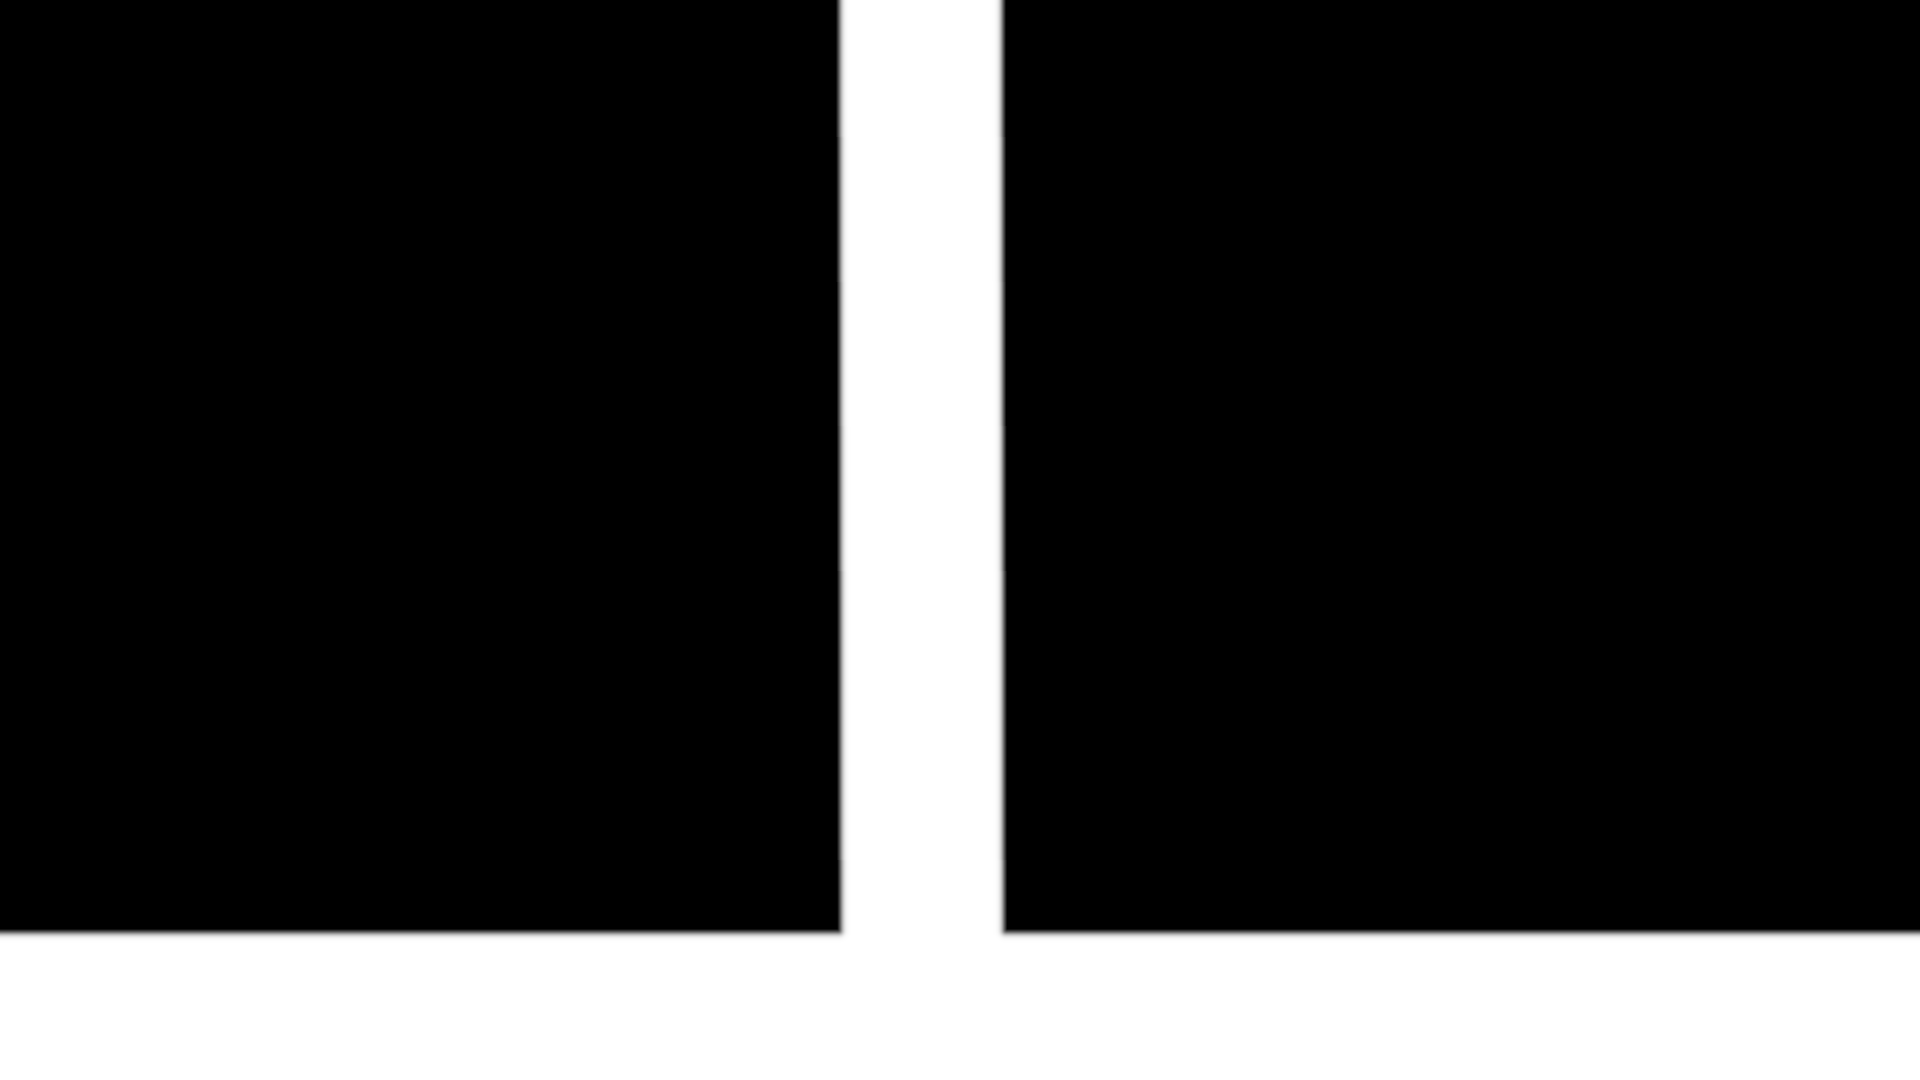
\includegraphics[width=.9\textwidth]{2_background/images/u_v_maps/example_1.png}}
		\caption{example 1}
	\end{subfigure}%
	\hfill
	\begin{subfigure}[t]{.45\textwidth}
		\centering
		\fcolorbox{black}{black}{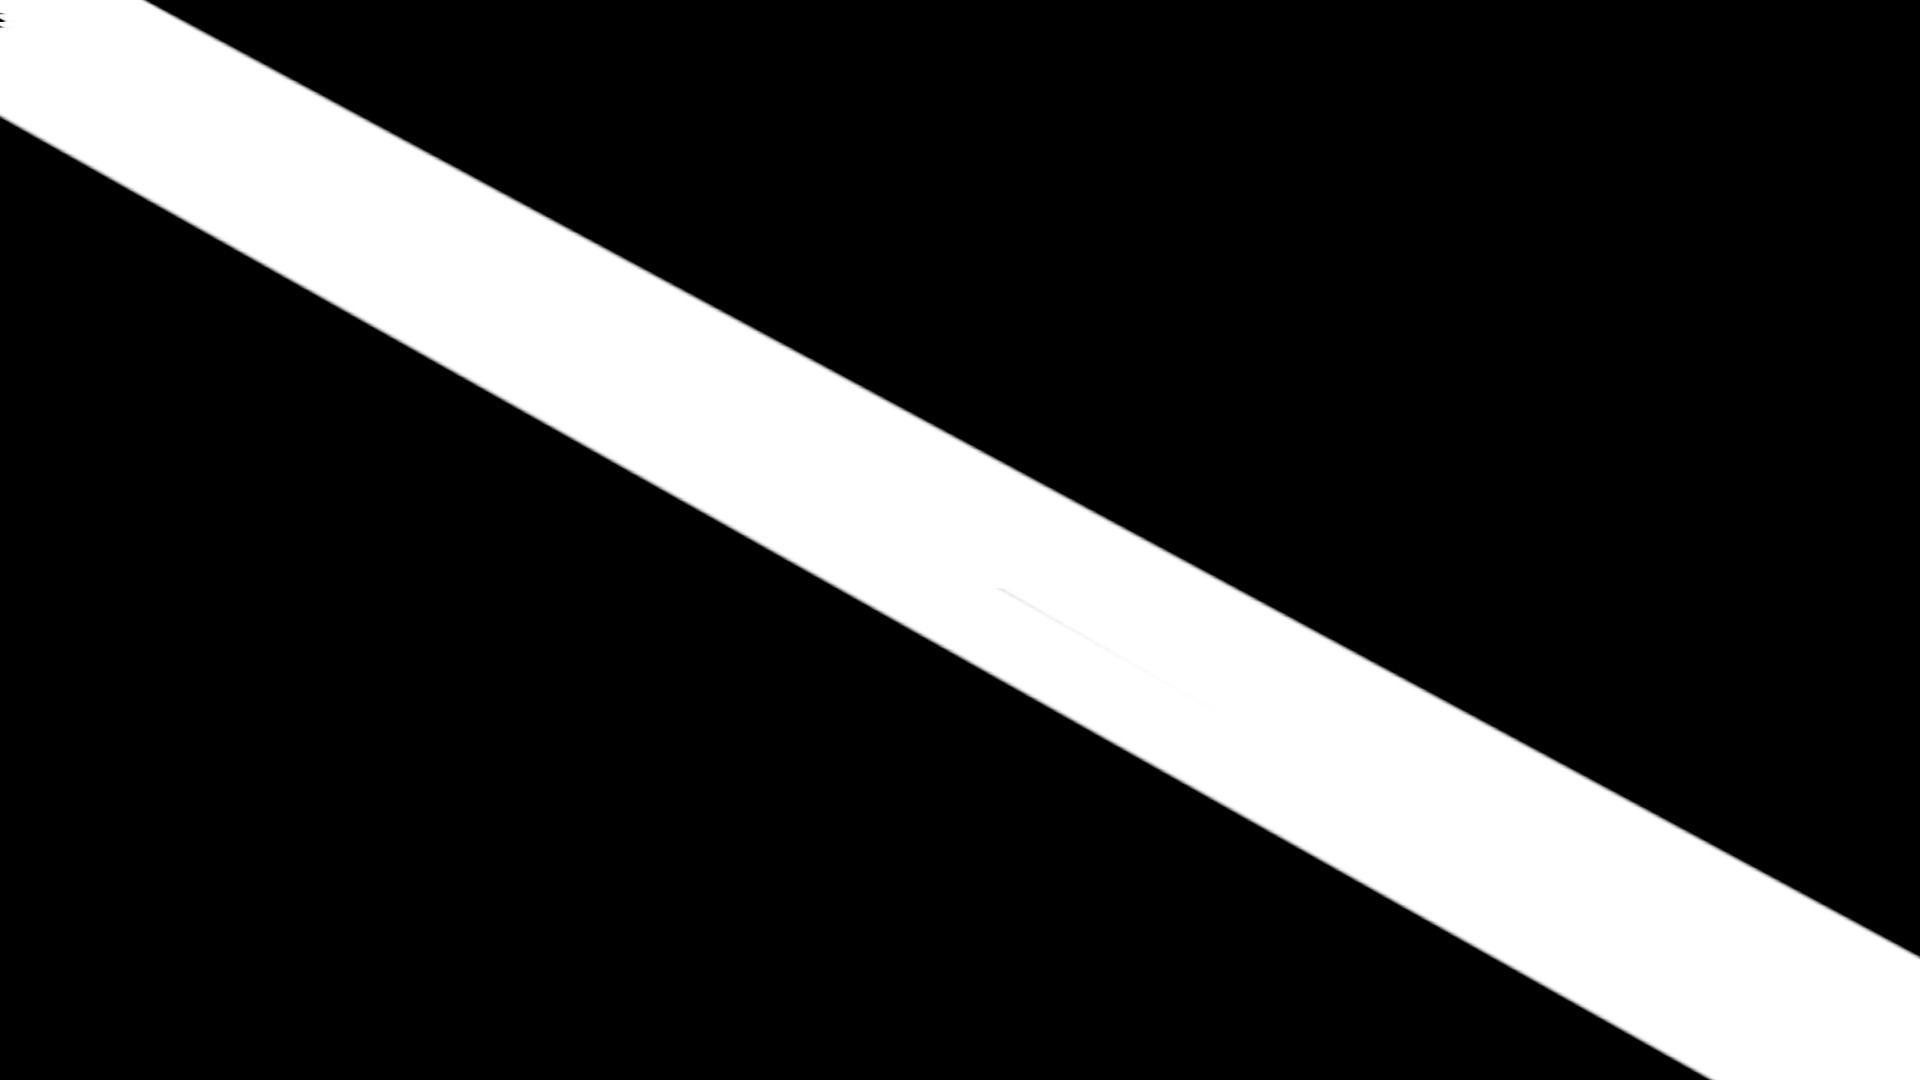
\includegraphics[width=.9\textwidth]{2_background/images/u_v_maps/example_2.png}}
		\caption{example 2}
	\end{subfigure}%
\caption{Two problematic situations for the U-V disparity approach are illustrated. The white color denotes the \textit{occupied} area and the black color denotes \textit{obstacle-free} area.}
\label{fig:U_V}
\end{figure} 


\subsubsection{Account for UAV Size and Find Pixels State}

After producing the image-space map, the \ac{UAV} needs to find the obstacle-free and occupied pixels in order to assess the risk of collision and subsequently perform path planning if necessary. In order to do so, the \ac{UAV} should be projected in the map assuming its projection center is the pixel in question, and check if the pixel(s) it ``touches" satisfy a minimum safe distance. There have been developed two main approaches so far:

%the risk of collision should be assessed in order to decide upon the requirement of a maneuver in case of a potential threat in front of the UAV. 

\begin{description}
	\item[Direct robot projection: ] The robot is directly projected to the image-space.
	\item[C-space expansion: ] Every pixel is expanded according to its disparity value and the robot is projected as a single point in the image-space.
\end{description}

In the \textit{direct robot projection} approach, Smith, et. al, model the robot directly in perception space \cite{Smith2017a}. In this study the drone's pose is projected in the depth image. While this idea has been tested in a ground robot, it will most probably not work for a UAV because of the rapid and continuous changes in vehicle's pose. An approximation of this method is to model the \ac{UAV} as a box or ellipse in the image space. In order to find the state of a pixel: The pixel should be considered \textit{obstacle-free} in case the pixels covered by the projection of the drone to the depth map have a disparity value lower than the disparity which corresponds to the projection depth. The center of the projection is the pixel which is under inspection. All projections depths that correspond to a distance equal or lower to the specified ``safe" distance should be examined. In case all the different projections are estimated to be safe, the pixel can be considered obstacle ``free". The computational complexity of this method in order to define all the \textit{obstacle-free} and \textit{occupied }pixels is $\Theta(\frac{L_x * L_y}{d_{min} * B}  * W * H)$, where L is the drone size, $d_{min}$ is the minimum disparity, B is the baseline, W is the with of the image and H is the height of the image.


The \textit{c-space expansion} approach (c-space stands for configuration space) projects the drone as a point in the image space. The origin of this idea came from Otte et.al.\cite{Otte2009} and has also been tested in a UAV \cite{Matthies2014}. Their base of the idea is the following: expand every pixel in the depth map according to the drone's dimensions and the pixel disparity/depth value. That way, the drone can just projected as a single point in the image. In order to find the state of a pixel: The pixel should be considered obstacle ``free" if its c-expanded value has a disparity lower than the disparity corresponding to the ``safe" distance. The c-expansion method has a computational complexity equal to $O(\frac{L_x * L_y}{d_{min} * B}  * W * H)$, where L is the drone size, $d_{min}$ is the minimum disparity, B is the baseline, W is the with of the image and H is the height of the image.

%Either of these methods should be used by the path planning component in order to generate an obstacle-free trajectory. Collision checking in a static environment is performed by examining if there are obstacles in front of the \ac{UAV} below a certain ``safe" distance. In case a collision is detected, an ``escape" trajectory should be planned on the image space by examining the \textit{obstacle-free} (pixels with depth value higher than the safe distance) and \textit{occupied} pixels. Consequently, it is obvious that knowledge of \textit{obstacle-free} and \textit{occupied} pixels is necessary.

Consequently, by calculating the computational complexity of both methods it is obvious that \textit{c-space expansion} has a potentially lower computational load and for this reason it should be preferred. 

\subsubsection{Collision Detection}

Collision detection in a static environment is a really simple process. After determining the \textit{obstacle-free} and \textit{occupied} pixels, a check on the pixel's state which corresponds to the center of the projection of the \ac{UAV} in the image space should be performed. In case it is found \textit{occupied} then a collision is detected. The (x,y) coordinates of the pixel can be calculated based on the following equations, where V is the \ac{UAV} speed and f is the focal length:

\begin{equation}\label{eq:x_col_check}
x = \frac{f}{V_z} * V_x
\end{equation}

\begin{equation}\label{eq:y_col_check}
y = \frac{f}{V_z} * V_y
\end{equation}


\subsubsection{Path planning in image space}
\label{ch:literature:state_of_the_art_avoidance:reactive_image_navigation:path_planning}


The only \ac{UAV} study that has experimented with path planning in image space is by Fragoso, et. al, \cite{Fragoso2017} but still they do not explain how the \textit{escape} points (obstacle-free image pixels) are calculated. Instead, they focus on the dynamics of the path planning. Our study proposes that path planning in image-space should be divided in two parts: 

\begin{enumerate}
	\item Trajectory planning when \ac{FoV} is not fully blocked.
	\item Trajectory planning when \ac{FoV} is fully blocked.
\end{enumerate} 

As a solution to the first step of image-space path planning, we propose a boundary tracing algorithm in order to find the boundary of the obstacle. Then the escape points will be all the points lying in this boundary. There are various boundary tracing algorithms, some examples are:

\begin{itemize}
    \item Square Tracing algorithm
    \item Moore-Neighbor Tracing algorithm
    \item Radial Sweep
    \item Theo Pavlidis’ algorithm
    \item Dr Kovalevsky algorithm
\end{itemize}{}

One of the most efficient algorithms among this list is Moore-Neighbor Tracing algorithm. After finding the escape points a cost function may assign a cost to each of them and the lowest cost escape point may be chosen as the best escape route for the UAV. A similar cost function has been used for ground robots experiments \cite{Ulrich1998} \cite{Borenstein1991} \cite{NALPANTIDIS2011a}. 

In case the image map is full of obstacles, no escape point exists in the \ac{FoV} of the \ac{UAV}. In case reaching a goal location is not a prerequisite, the \ac{UAV} should hover and rotate until its \ac{FoV} is not anymore blocked. Then the boundary tracing algorithm can be executed to calculate the escape points. 

In case reaching a goal state is a prerequisite, the only low-cost method found in literature is the usage of a bug algorithm. However, most of them have not been designed to be used with a vision sensor. An exception to this is \cite{laubach1999autonomous} which presents a bug algorithm specifically designed for a stereo-based rover. It is a variation of the classic tangent bug algorithm \cite{kamon1996new}. Its concept is as follows: When no decision can be taken based on the image map, the robot should change its mode from Motion-to-Goal to Boundary-Following. As the name suggests, with the Boundary Following function the robot is able to skirt the obstacle until a stopping criterion change its mode again from Boundary-Following to Motion-to-Goal. Usually this stopping criterion is when further progress towards a goal location can be made. Here, it is worthwhile noting a difference between the localization needs of image-space planning and the localization needs of discretized planning. The first one needs to find only the distance and azimuth angle to the goal localation according to \cite{mcguire2019comparative}. The latter one needs accurate position estimation in order to merge information from different time measurements. 

\subsubsection{Dynamics}

After generating the UAV's avoidance trajectory, there is a chance that the potential required maneuver may not be feasible under the current UAV velocity. The inclusion of dynamics make sure that the generated path can be executed by the drone. 

There is only one study in image-space planning which includes dynamics in its trajectory generation \cite{Fragoso2017}. After identifying an infeasible candidate path, their method tries to smoothly transform it into a feasible maneuver. Their receding-horizon approach does not guarantee completeness and may stuck in dead ends. However, is it the fastest existing method so far and ideal for image-space mapping. 

\section{Conclusion}

In this chapter, necessary obstacle avoidance terminology was introduced. Moreover an overview was given of the state-of-the-art stereo algorithms used in low-cost UAV obstacle avoidance studies so far. Finally, an attempt to classify the different collision avoidance approaches and a review of the existing image-based avoidance methods was presented. In the next chapter, a new innovative idea will be introduced, a method that takes into account the uncertainty in environment sensing, which is naturally inherent in any stereo algorithm.

